%=========================================================
\chapter{Modelo del Negocio}	
\label{cap:reqSist}

	En este capítulo se modela la {\em Arquitectura del negocio} la cual está conformada por los ({\em Términos} y {\em Hechos del negocio}), Arquitectura de procesos y las {\em Reglas del negocio}. Primero se especifica brevemente el {\em Contexto} en el que los términos tienen significado.
	
%----------------------------------------------------------
\section{Contexto}

%	\cdtInstrucciones{El contexto debe explicar bajo que ambiente los términos del negocio son aplicables y proporcionar información general para su comprensión inicial.\\}
	Consorcio Deportivo S.A. de C.V.  es una empresa nueva, que busca crecer a nivel nacional, para esto se unió con otras cadenas deportivas. Al poner en funcionamiento sus gimnasios en Monterrey, Guadalajara y en la Ciudad de México, se dieron cuenta que las demás cadenas tienen procesos, procedimientos e información diferentes; algunas personas que viajan y que quieren seguir con su rutina de ejercicio, se les negó el ingreso a las instalaciones ya que la información no se encuentra unificada en todas las sucursales.
	
	Las actividades que pueden ser contratadas tienen problemas ya que no tienen control alguno. Estas actividades son: área de piscina, área de instrumentos (pesas, caminadoras, etc.), área de canchas (fútbol, tennis, etc.).  De igual manera las membresías carecen de control alguno, ya que los miembros no ponen atención a la fecha de renovación de estas. Los miembros a los que se les notificó que tenían su pago de renovación atrasado se les negaba su ingreso a lo que el miembro se respalda tras la escusa que ya realizó el pago, ya que no hay manera de comprobar de manera inmediata la veracidad de esto, se le da acceso al cliente, esto se traduce en pérdidas.
	
%---------------------------------------------------------
\section{Términos del Negocio}
\label{sec:terminosDeNegocio}

\begin{description}
	% Ejemplo de un término literal.
	%\item[\hypertarget{tAutomovil}{Automóvil:}] ({\em es un tipo de \hyperlink{tVehiculo}{Vehículo}}) De cuatro ruedas con capacidad de 5 a 9 personas. 
	% Ejemplo de un término de entidad
	%\item[\hypertarget{tCliente}{Cliente:}] Se refiere a todas las personas físicas y morales que \hyperlink{tRenta}{rentan} o han rentado un \hyperlink{tVehiculo}{vehículo}.
	
	\item[\hypertarget{tDirector}{Director:}] ({\em es un tipo de \hyperlink{tEmpleado}{Empleado}}) Es el empleado que tiene mayor rango de todos y no tiene superior, a diferencia de los demás.	
	\item[\hypertarget{tEmpleado}{Empleado:}] Se refiere a cualquier persona que labore en la empresa.
	 
	\item[\hypertarget{tChecador}{Checador:}] ({\em Reloj asociado al atributo:} Hora de entrada y salida de un \hyperlink{tEmpleado}{empleado}. {\em Frecuencia de lectura:} Una vez al día para la entrada y otra para la salida durante los días laborales.
	
	\item[\hypertarget{tMotocicleta}{Motocicleta:}] ({\em es un tipo de {tVehiculo}{Vehículo}}) De dos ruedas con capacidad para una personas. 

	\item[\hypertarget{tRenta}{Renta:}] Se refiere al servicio que ofrece la empresa para prestar \hyperlink{tVehiculo}{vehículos} a los \hyperlink{tCliente}{clientes} por un tiempo definido.
	
	\item[\hypertarget{tVehiculo}{Vehiculo:}] Se refiere a los automóviles y motocicletas que la empresa usa para dar el servicio de renta a los \hyperlink{tCliente}{clientes}.
	
%	\brTermSensor{tVelocimetro}{Velocímetro:}{Velocidad de un Vehículo.}{Kilometros/hora.}{Constantemente siempre que el \cdtRef{tVehiculo}{vehículo} esté encendido.}
\end{description}

%----------------------------------------------------------
\section{Modelo del dominio del problema}
\label{sec:hechosDeNegocio}


%- - - - - - - - - - - - - - - - - - - - - - - - - - - - - 
\subsection{Modelo del dominio del problema}

	El modelo del dominio del problema se muestra en la figura~\ref{fig:modeloDeDominio}, a continuación se describen cada una de las entidades y sus relaciones.
	
\begin{figure}[htbp!]
	\begin{center}
		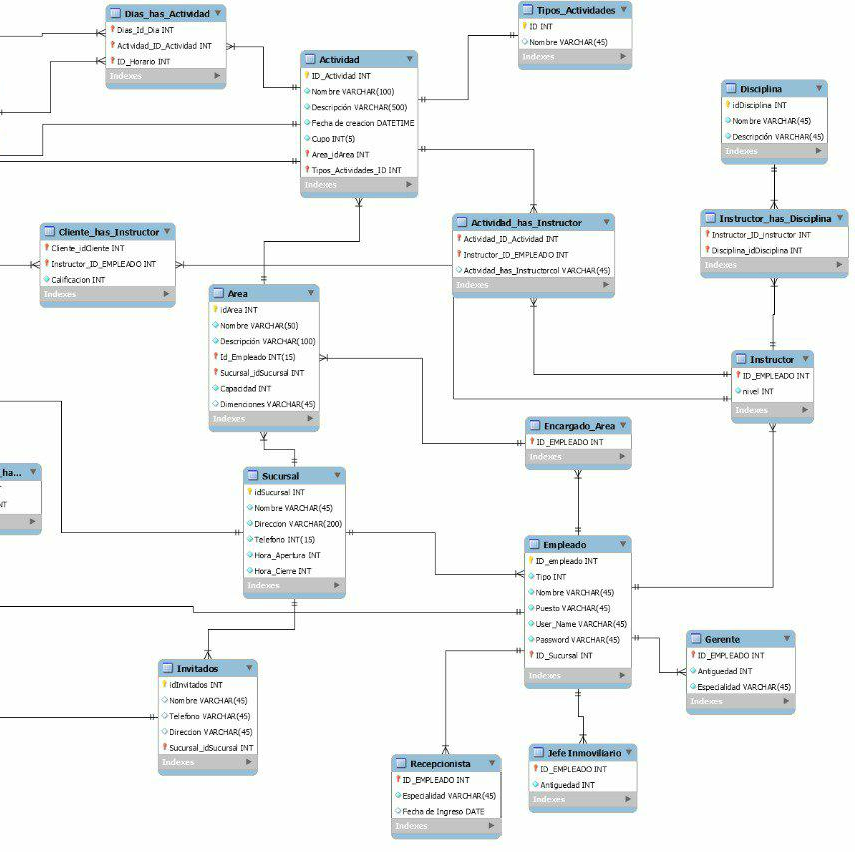
\includegraphics[angle=90,width=.95\textwidth]{images/modeloDelDominioDelProblema1}
		\caption{Modelo del dominio del problema parte 1}
		\label{fig:modeloDeDominio}
	\end{center}
\end{figure}

\begin{figure}[htbp!]
	\begin{center}
		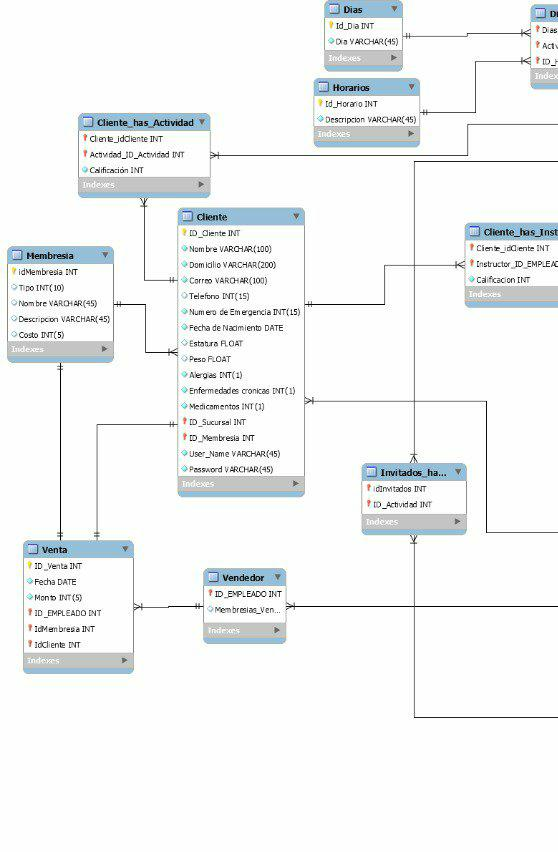
\includegraphics[angle=90,width=.95\textwidth]{images/modeloDelDominioDelProblema2}
		\caption{Modelo del dominio del problema parte 1}
		\label{fig:modeloDeDominio}
	\end{center}
\end{figure}

%- - - - - - - - - - - - - - - - - - - - - - - - - - - - - 

\newenvironment{cdtEntidad}[2]{%
	\def \varBusinessEntityId{#2}%
	\hypertarget{#1}{\hspace{1pt}}%
	\newline%
	\noindent{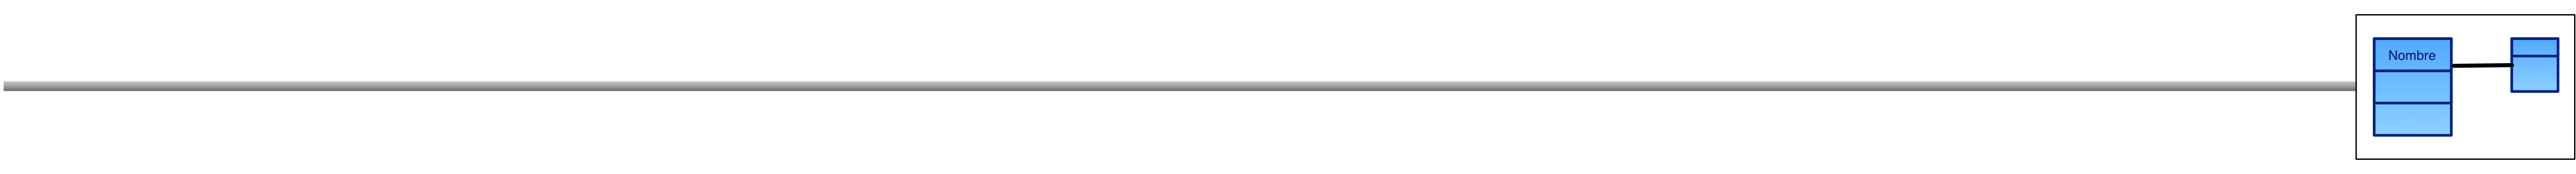
\includegraphics[width=\textwidth]{images/uc/classRule}}%
	\vspace{-25pt}%
	\subsection{Entidad: #2}%
	\noindent\begin{longtable}{|p{.2\textwidth}| p{.15\textwidth} | p{.46\textwidth} |p{.08\textwidth} |}%
		\hline%
		\multicolumn{4}{|c|}{{\cellcolor{colorSecundario}\color{white}Atributos}}\\ \hline%
		{\cellcolor{colorAgua}Nombre} &%
		{\cellcolor{colorAgua}Tipo} &%
		{\cellcolor{colorAgua}Descripción} &%
		{\cellcolor{colorAgua}Requerido}%
		\\ \hline%
		\endhead%
	}{%
	\end{longtable}%
}

\newcommand{\brAttr}[5]{%
	{\bf\hypertarget{\varBusinessEntityId:#1}{#2}} & {\em{#3}} & {#4} & #5 \\\hline
}

\newcommand{\cdtEntityRelSection}{%
	\multicolumn{4}{|c|}{{\cellcolor{colorSecundario}\color{white}Relaciones}}\\ \hline%
	{\cellcolor{colorAgua}Tipo de relación} &%
	{\cellcolor{colorAgua}Entidad} &%
	\multicolumn{2}{|c|}{{\cellcolor{colorAgua}Rol}}
	\\ \hline%
}

\newcommand{\brRelComposition}{{\color{colorPrincipal}$\Diamondblack$\hspace{-1pt}---Composición}}
\newcommand{\brRelAgregation}{{\color{colorPrincipal}$\Diamond$\hspace{-1pt}---Agregación}}
\newcommand{\brRelGeneralization}{{\color{colorPrincipal}$\lhd$\hspace{-1pt}---Generalización}}

\newcommand{\brRel}[3]{%
	{\em{#1}} & {\bf{#2}} & \multicolumn{2}{|l|}{#3}\\\hline
}

%- - - - - - - - - - - - - - - - - - - - - - - - - - - - - 

\begin{cdtEntidad}{Cliente}{Cliente}
	\brAttr{Cliente}{Cliente}{Id}{Número de registro para identificar al cliente.}{Sí}
	\brAttr{nombre}{Nombre}{Palabra larga}
	{Nombrecompleto del cliente.}{Sí}
	\brAttr{Domicilio}{Domicilio}{Palabra }
	{Domicilio del cliente.}{Sí}
	\brAttr{Correo}{Correo}{Correo}{Correo del cliente para envio de circulares o avisos.}{No}
	\brAttr{Telefono}{Telefono}{Telefono}{Telefono de contacto del cliente}{No}
	\brAttr{NumeroEmergencia}{Numero de emergencia}{Telefono}
	{Telefono de contcto en caso de alguna emergencia.}{Sí}
	\brAttr{nacimiento}{Nacimiento}{Fecha}
	{Fecha de nacimiento del cliente.}{Sí}
	\brAttr{Estatura}{Estatura}{Flotante}{Estatura del cliente}{NO}
	\brAttr{Peso}{Peso}{Flotante}
	{Peso del cliente.}{NO}
	\brAttr{Alergias}{Alergias}{Booleano}
	{Si el cliente cuenta con alguna alergia.}{Sí}	
	\brAttr{Enfermedades}{Enfermedades}{Booleano}
	{Si el cliente cuenta con alguna enfermedad crónica.}{SI}
	\brAttr{Medicación}{Medicación}{Booleano}
	{Si el cliente cuenta con medicación.}{SI}
	\brAttr{sucursal}{sucursal}{ID}{Numero de registro para identificar la sucursal a la que pertenece}{SI}
	\brAttr{ID_Membresia}{Membresía}{ID}
	{Numero de registro para identificar la membresia qye tiene el cliente.}{SI}
	\brAttr{Nombre}{Usuario}{Nombre de y usuario}{Nombre de usuario para iniciar sesion}{SI}
	
	\cdtEntityRelSection
	\brRel{\brRelGeneralization}{Empleado}{Un \hyperlink{Gerente}{Gerente} es un \hyperlink{Empleado}{Empleado}}	
\end{cdtEntidad}
%- - - - - - - - - - - - - - - - - - - - - - - - - - - - - 

\begin{cdtEntidad}{Gerente}{Gerente}
	\brAttr{Empleado}{Empleado}{Id}{Número de registro para identificar al empleado.}{Sí}
	\brAttr{Antigedad}{Antigedd}{Entero Corto}
	{Antigedad en la Sucursal.}{Sí}
	\brAttr{Domicilio}{Domicilio}{Palabra }
	{Domicilio del cliente.}{Sí}
	
	
	\cdtEntityRelSection
	\brRel{\brRelComposition}{Sucursal}{Un \hyperlink{Cliente}{Cliente} pertenece a una \hyperlink{Sucursal}{Sucursal}}	
	\brRel{\brRelAgregation}{Membresía}{Un \hyperlink{Cliente}{Cliente} tiene una \hyperlink{Membresia}{Membresia}}	
\end{cdtEntidad}
%- - - - - - - - - - - - - - - - - - - - - - - - - - - - - 

\begin{cdtEntidad}{Instructor}{Instructor}
	\brAttr{Empleado}{ID}{Id}{Número de registro para identificar al empleado.}{Sí}
	\brAttr{Nivel}{Nombre}{entero corto}
	{Nivel en el que se encuentra en la sucurusal.}{Sí}
	
	
	\cdtEntityRelSection
	\brRel{\brRelGeneralization}{Empleado}{Un \hyperlink{Instructor}{Instructor} es un \hyperlink{Empleado}{Empleado}}	
\end{cdtEntidad}


%- - - - - - - - - - - - - - - - - - - - - - - - - - - - - 

\begin{cdtEntidad}{Recepcionista}{Recepcionista}
	\brAttr{Empleado}{ID}{Id}{Número de registro para identificar al empleado.}{Sí}
	\brAttr{Especialidad}{Especialidad}{Nombre corto}
	{Especialidad de la recepcionista en alguna área.}{Sí}
	
	
	\cdtEntityRelSection
	\brRel{\brRelGeneralization}{Empleado}{Un \hyperlink{Recepcionista}{Recepcionista} es un \hyperlink{Empleado}{Empleado}}	
\end{cdtEntidad}

%- - - - - - - - - - - - - - - - - - - - - - - - - - - - -

\begin{cdtEntidad}{Vendedor}{Vendedor}
	\brAttr{Empleado}{ID}{Id}{Número de registro para identificar al empleado.}{Sí}
	\brAttr{Membresias}{Venta}{entero corto}
	{Numero de membresias vendidas desde su ingreso.}{NO}
	
	
	\cdtEntityRelSection
	\brRel{\brRelGeneralization}{Empleado}{Un \hyperlink{Recepcionista}{Recepcionista} es un \hyperlink{Empleado}{Empleado}}	
\end{cdtEntidad}

%- - - - - - - - - - - - - - - - - - - - - - - - - - - - -

\begin{cdtEntidad}{Sucursal}{Sucursal}
	\brAttr{Sucursal}{Sucursal}{Id}{Número de registro para identificar una sucursal.}{Sí}
	\brAttr{nombre}{Nombre}{Palabra corta}
	{Nombrecompleto de la sucursal.}{Sí}
	\brAttr{Domicilio}{Domicilio}{Palabra larga}
	{Domicilio de la sucursal.}{Sí}
	\brAttr{Telefono}{Telefono}{Telefono}{Telefono de contacto para la sucursal}{SI}
	\brAttr{Hora}{Apertura}{hora}{Hora en la que empieza a dar servicio la sucursal}{SI}
	\brAttr{Hora}{Cierre}{hora}
	{hora en la que se termina el sevicio en la sucursal.}{SI}
	
\end{cdtEntidad}
%- - - - - - - - - - - - - - - - - - - - - - - - - - - - - 

\begin{cdtEntidad}{Venta}{Venta}
	\brAttr{ID}{Venta}{Id}{Número de registro para identificar la venta.}{Sí}
	\brAttr{Fecha}{Fecha}{fecha}
	{Fecha en la que se realizo la venta.}{Sí}
	\brAttr{Monto}{Monto}{Flotante }
	{Monto de la venta.}{Sí}
	\brAttr{ID}{Empleado}{ID}{Numero de registro para identificar el empleado que vendio la membresia}{si}
	
	
	\cdtEntityRelSection
	\brRel{\brRelComposition}{Vendedor}{Una \hyperlink{Venta}{Venta} tiene un \hyperlink{Vendedor}{Vendedor} que realizó la venta}	
	\brRel{\brRelComposition}{Membresía}{Una \hyperlink{Venta}{Venta} tiene una \hyperlink{Membresia}{Membresia} asignada}
	\brRel{\brRelComposition}{Cliente}{Ua \hyperlink{Venta}{Venta} tiene un \hyperlink{Cliente}{Cliente} que la solicitó}	
\end{cdtEntidad}
%---------------------------------------------------------

	\begin{cdtEntidad}{Actividad}{Actividad}
	\brAttr{ID}{Actividad}{Id}{Número de registro para identificar la Actividad.}{Sí}
	\brAttr{Nombre}{Nombre}{Nombre corto}
	{Nombre de la actividad.}{Sí}
	\brAttr{Descripcion}{Descripcion}{Nombre largo}
	{Descripcion de la actividad.}{Sí}
	\brAttr{Fecha}{Creacion}{fecha}{Fecha en la que se creo la Actividad}{SI}
	\brAttr{Cupo}{Cupo}{Entero}{Cupo máximo de la actividad}{SI}
	\brAttr{ID}{Area}{ID}{Numero de registro para identificar el area a la que pertenece la actividad}{SI}
	\brAttr{ID}{Actividad}{ID}{Numero de registro para identificar el tipo de actividad}{SI}
	
	\cdtEntityRelSection
	\brRel{\brRelComposition}{Area}{Una \hyperlink{Actividad}{Actividad} tiene un \hyperlink{Area}{Area} asignada}	
	\brRel{\brRelComposition}{TipoActividad}{Una \hyperlink{Actividad}{Actividad} tiene un \hyperlink{TipoActividad}{TipoActividad}}	
\end{cdtEntidad}

%---------------------------------------------------------

\begin{cdtEntidad}{Area}{Area}
	\brAttr{ID}{Area}{Id}{Número de registro para identificar un area.}{Sí}
	\brAttr{Nombre}{Nombre}{Nombre corto}
	{Nombre del area.}{Sí}
	\brAttr{Descripcion}{Descripcion}{Nombre largo}
	{Descripcion del area.}{Sí}
	\brAttr{ID}{Empleado}{ID}{Numero de registro para identificar al encargado de área}{SI}
	\brAttr{ID}{Sucursal}{ID}{Numero de registro para identificar la sucursal a la que pertenece}{SI}
	\brAttr{Capacidad}{Capacidad}{Numerico}{Numero de personas que pueden estar en el area}{SI}
	\brAttr{Dimensiones}{Dimensiones}{Nombre corto}{Metros de largo por metros de ancho}{SI}
	\cdtEntityRelSection
	\brRel{\brRelAgregation}{Encargado}{Un \hyperlink{Area}{Area} tiene un \hyperlink{Encargado}{Encargado} asignada}	
	\brRel{\brRelComposition}{Sucursal}{Un \hyperlink{Area}{Area} pertenece a una \hyperlink{Sucursal}{Sucursal}}	
	\end{cdtEntidad}
	
	%---------------------------------------------------------
\section{Modelado de Reglas de negocio}

\begin{BussinesRule}{BR1}{Cortesía de acceso.}
	\BRitem[Tipo:] Regla de integridad referencial o estructural. 
				% Otras opciones para tipo: 
				% - Regla de integridad referencial o estructural. 
				% - Regla de operación, (calcular o determinar un valor.).
				% - Regla de inferencia de un hecho.
	\BRitem[Clase:] Habilitadora. 
				% Otras opciones para clase: Habilitadora, Cronometrada, Ejecutive.
	\BRitem[Nivel:] Control. % Otras opciones para nivel: Control, Influencia.
	\BRitem[Descripción:]	Si una persona no registrada en los clubs solicita una cortesía, se le registrara en el sistema y se le dará acceso por una solo única vez sin posibilidad de repetición..
	\BRitem[Motivación:] Para generar ventas de membresía.
	%\BRitem[Sentencia:] $\forall p \in Persona \Rightarrow 01-Enero-1900~<~p.fechaDeNacimiento~<~fechaActual$.
	\BRitem[Ejemplo positivo:] Para personas que no estén registradas en el sistema, cumplen la regla: 		
        	
	\BRitem[Ejemplo negativo:] Para quienes aparece su nombre en el sistema, no cumplen la regla.
	
	\BRitem[Referenciado por:] %\hyperlink{CUCE3.2}{CUCE3.2}, \hyperlink{CUCE3.3}{CUCE3.3}.
\end{BussinesRule}

\begin{BussinesRule}{BR2}{Límite de personas en Membresía Familiar.} 
	\BRitem[Tipo:] Regla de integridad referencial o estructural. 
				% Otras opciones para tipo: 
				% - Regla de integridad referencial o estructural. 
				% - Regla de operación, (calcular o determinar un valor.).
				% - Regla de inferencia de un hecho.
	\BRitem[Clase:] Cronometrada. 
				% Otras opciones para clase: Habilitadora, Cronometrada, Ejecutive.
	\BRitem[Nivel:] Control. % Otras opciones para nivel: Control, Influencia.
	\BRitem[Descripción:] Al adquirir una membresía familiar el número máximo de usuarios que se pueden registrar para la entrada a las sucursales es de 10 personas sin distinción de edad y sin remplazo.
	\BRitem[Ejemplo positivo:] Para familias con menos de 11 de integrantes, cumplen la regla:
		\begin{itemize}
			\item Familias con 10 integrantes
			\item Familias con 9 integrantes
			\item .
			\item .
			\item .
			\item Familias con 2 integrantes
			contenidos...
		\end{itemize}
	
	\BRitem[Ejemplo negativo:] Familias que quieran adquirir la membresia con integrantes de mas de 10 personas, no cumplen la regla:
		\begin{itemize}
			\item Familias con 11 integrantes
			\item Familias con 15 integrantes
			contenidos...
		\end{itemize}
	
	\BRitem[Referenciado por:] 
\end{BussinesRule}

\begin{BussinesRule}{BR3}{Acceso a la sucursal}
	\BRitem[Tipo:] Regla de integridad referencial o estructural.
				% Otras opciones para tipo: 
				% - Regla de integridad referencial o estructural. 
				% - Regla de operación, (calcular o determinar un valor.).
				% - Regla de inferencia de un hecho.
	\BRitem[Clase:] Habilitadora. 
				% Otras opciones para clase: Habilitadora, Cronometrada, Ejecutive.
	\BRitem[Nivel:] Control. % Otras opciones para nivel: Control, Influencia.
	\BRitem[Descripción:] Si se desea ingresar a cualquier sucursal, el acceso es único con membresía, si no cuenta con una puede consultar la RB1, de alguna otra forma se reserva el derecho de admisión.
	\BRitem[Ejemplo positivo:] Aquellos que tengan su membresía, cumplen con la regla:
		\begin{itemize}
			\item Presenta su membresía a la recepcionista.
			\item Presenta su correo a la recepcionista.
			contenidos...
		\end{itemize}
	
	\BRitem[Ejemplo negativo:] Aquellas personas que no traigan su membresía o no esten registrados en el sistema, no cumplen con la regla:
		\begin{itemize}
			\item Presenta correo no registrado
			\item Presenta membresía vencida por mas de 1 semana.
			contenidos...
		\end{itemize}
	
	\BRitem[Referenciado por:] 
\end{BussinesRule}

\begin{BussinesRule}{BR5}{Acceso a Actividades}
	\BRitem[Tipo:] Regla de integridad referencial o estructural.
				% Otras opciones para tipo: 
				% - Regla de integridad referencial o estructural. 
				% - Regla de operación, (calcular o determinar un valor.).
				% - Regla de inferencia de un hecho.
	\BRitem[Clase:] Habilitadora. 
				% Otras opciones para clase: Habilitadora, Cronometrada, Ejecutive.
	\BRitem[Nivel:] Control. % Otras opciones para nivel: Control, Influencia.
	\BRitem[Descripción:] El acceso a cada actividad está sujeto al tipo de membresía con el cual se cuenta o se contrató, no es posible acceder a una actividad que no este referenciada en la membresía contratada a menos que sea pagada de forma individial.
	\BRitem[Ejemplo positivo:] Cumplen la regla aquellos que en su tipo de membresía les permita a acceder a ciertas actividades:
		\begin{itemize}
			\item Membresía Familiar ingresa a las canchas y algunas actividades.
			 \item Membresía Premium ingresa a todas las actividades de la sucursal.
		\end{itemize}
	
	\BRitem[Ejemplo negativo:] 
	
	\BRitem[Referenciado por:] 
\end{BussinesRule}

\begin{BussinesRule}{BR6}{Adquisición de Membresías}
	\BRitem[Tipo:] Regla de integridad referencial o estructural.
				% Otras opciones para tipo: 
				% - Regla de integridad referencial o estructural. 
				% - Regla de operación, (calcular o determinar un valor.).
				% - Regla de inferencia de un hecho.
	\BRitem[Clase:] Habilitadora. 
				% Otras opciones para clase: Habilitadora, Cronometrada, Ejecutive.
	\BRitem[Nivel:] Control. % Otras opciones para nivel: Control, Influencia.
	\BRitem[Descripción:] Un usuario puede tener un único tipo de membresía acorde a sus necesidades.
	%\BRitem[Sentencia:] $Impuesto(e, s) = Costo(e, s)\cdot0.16$.
	\BRitem[Ejemplo positivo:] Al conmprar una membresía cumplen la regla:
		\begin{itemize}
			\item Personas que cambien de membresía.
			\item Personas que no tengan membresía.
		\end{itemize}
	
	\BRitem[Ejemplo negativo:] 
		\begin{itemize}
			\item Personas que no quieran renovar su membresía y quieran adquirir una doble membresía.
			\item Personas que no efectuen su pago.
			
		\end{itemi}
	
	\BRitem[Referenciado por:] 
\end{BussinesRule}

\begin{BussinesRule}{BR7}{Acceso a personas con retrazos en pagos.}
	\BRitem[Tipo:] Regla de integridad referencial o estructural.
				% Otras opciones para tipo: 
				% - Regla de integridad referencial o estructural. 
				% - Regla de operación, (calcular o determinar un valor.).
				% - Regla de inferencia de un hecho.
	\BRitem[Clase:] Habilitadora. 
				% Otras opciones para clase: Habilitadora, Cronometrada, Ejecutive.
	\BRitem[Nivel:] Control. % Otras opciones para nivel: Control, Influencia.
	\BRitem[Descripción:] Si un cliente no genera su pago par mas de una semana, al ingreso a la sucursal la secretaria indica que debe realizar su pago a la brevedad, tomando en cuenta que el próximo ingreso se le negara.
	%\BRitem[Sentencia:] $CostoTotal = Costo(e, s) + Impuesto(e, s)$.
	\BRitem[Ejemplo positivo:] El cliente que no relice su pago, cumplira la regla:
		\begin{itemize}
			\item Personas con mas de una semana sin realizar pago no entra a la sucursal.
			\item Clientes que tengan menos de una semana sin pagar la membresía podrán acceder.
		\end{itemize}
	
	\BRitem[Ejemplo negativo:] 
		\begin{itemize}
			\item Personas que si pagen su membresía a tiempo si entran a al sucursal
		\end{itemize}
	
	\BRitem[Referenciado por:] 
\end{BussinesRule}



%---------------------------------------------------------
\section{Modelo de Procesos AS-IS}

En esta sección se describen los procesos a mejorar con el sistema.

%%%%% - - - - - - - - - - - - - - - - - - - - - - - - - - - - 
\subsection{PROC-01 Análisis de requerimientos}

\begin{figure}[htbp]
	\begin{center}
		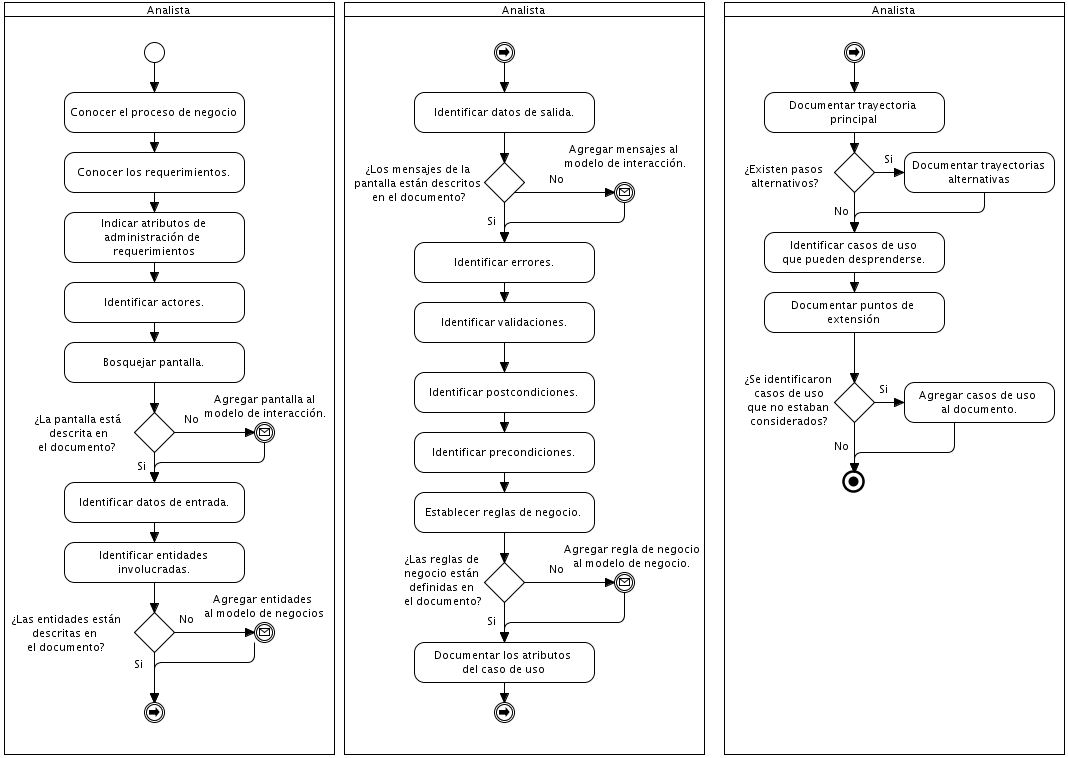
\includegraphics[width=.7\textwidth]{images/proceso1}
		\caption{PROC-01 Proceso de Análisis de requerimientos}
		\label{fig:proceso1}
	\end{center}
\end{figure}

\begin{description}
	\item[Descripción:] Describa el proceso indicando los aspectos relevantes que el diagrama no muestra.
	\item[Entradas:] \cdtEmpty
        \begin{itemize}
			\item Documentos de Procesos.
			\item Reglas de negocio.
			\item Minutas de las reuniones de análisis.
        \end{itemize}
	\item[Salidas:] \cdtEmpty
        \begin{itemize}
			\item Especificación de requerimientos.
			\item Bosquejo de pantallas.
			\item Modelo de base de datos
        \end{itemize}	
    \item[Áreas de oportunidad:] Liste los aspectos que detecta se pueden mejorar con la introducción del sistema o los problemas encontrados.
\end{description}

%%%%% - - - - - - - - - - - - - - - - - - - - - - - - - - - - 
\subsection{PROC-02 ...}

\begin{figure}[htbp]
	\begin{center}
		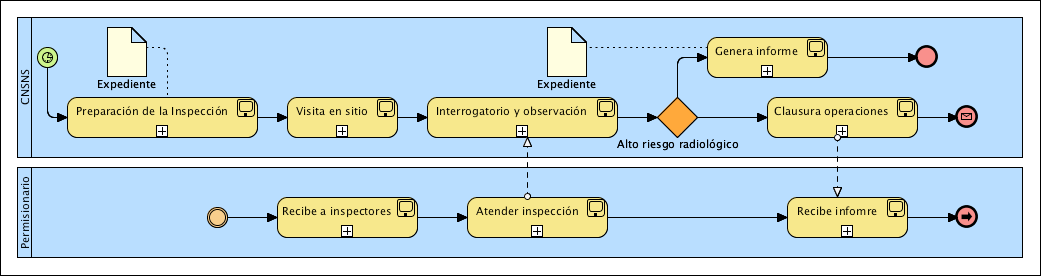
\includegraphics[width=.8\textwidth]{images/proceso2}
		\caption{PROC-02 Nombre del proceso}
		\label{fig:proceso2}
	\end{center}
\end{figure}

\begin{description}
	\item[Descripción:] ...
	\item[Entradas:] \cdtEmpty
        \begin{itemize}
			\item ...
        \end{itemize}
	\item[Salidas:] \cdtEmpty
        \begin{itemize}
			\item ...
        \end{itemize}	
    \item[Áreas de oportunidad:] Liste los aspectos que detecta se pueden mejorar con la introducción del sistema o los problemas encontrados.
\end{description}


%\input{proc/proc03.tex}
%\input{proc/proc04.tex}

%---------------------------------------------------------
\section{Modelo de procesos TO-BE}

Los nuevos procesos se presentan en esta sección, el mapa de procesos de se muestra en la figura~\ref{fig:mapaProc}.

\begin{figure}[htbp]
	\begin{center}
		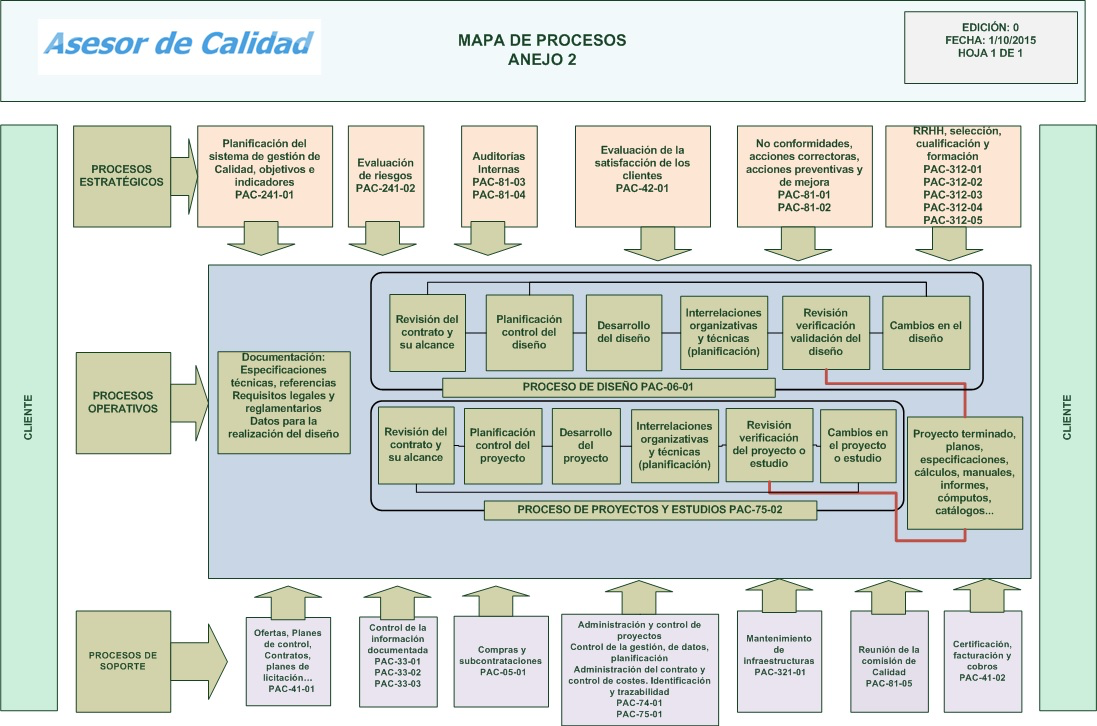
\includegraphics[width=.8\textwidth]{images/mapaProc}
		\caption{Mapa de procesos}
		\label{fig:mapaProc}
	\end{center}
\end{figure}


% - - - - - - - - - - - - - - - - - - - - - - - - - - - - 
\subsection{PROCM-01 ...}

\begin{figure}[htbp]
	\begin{center}
		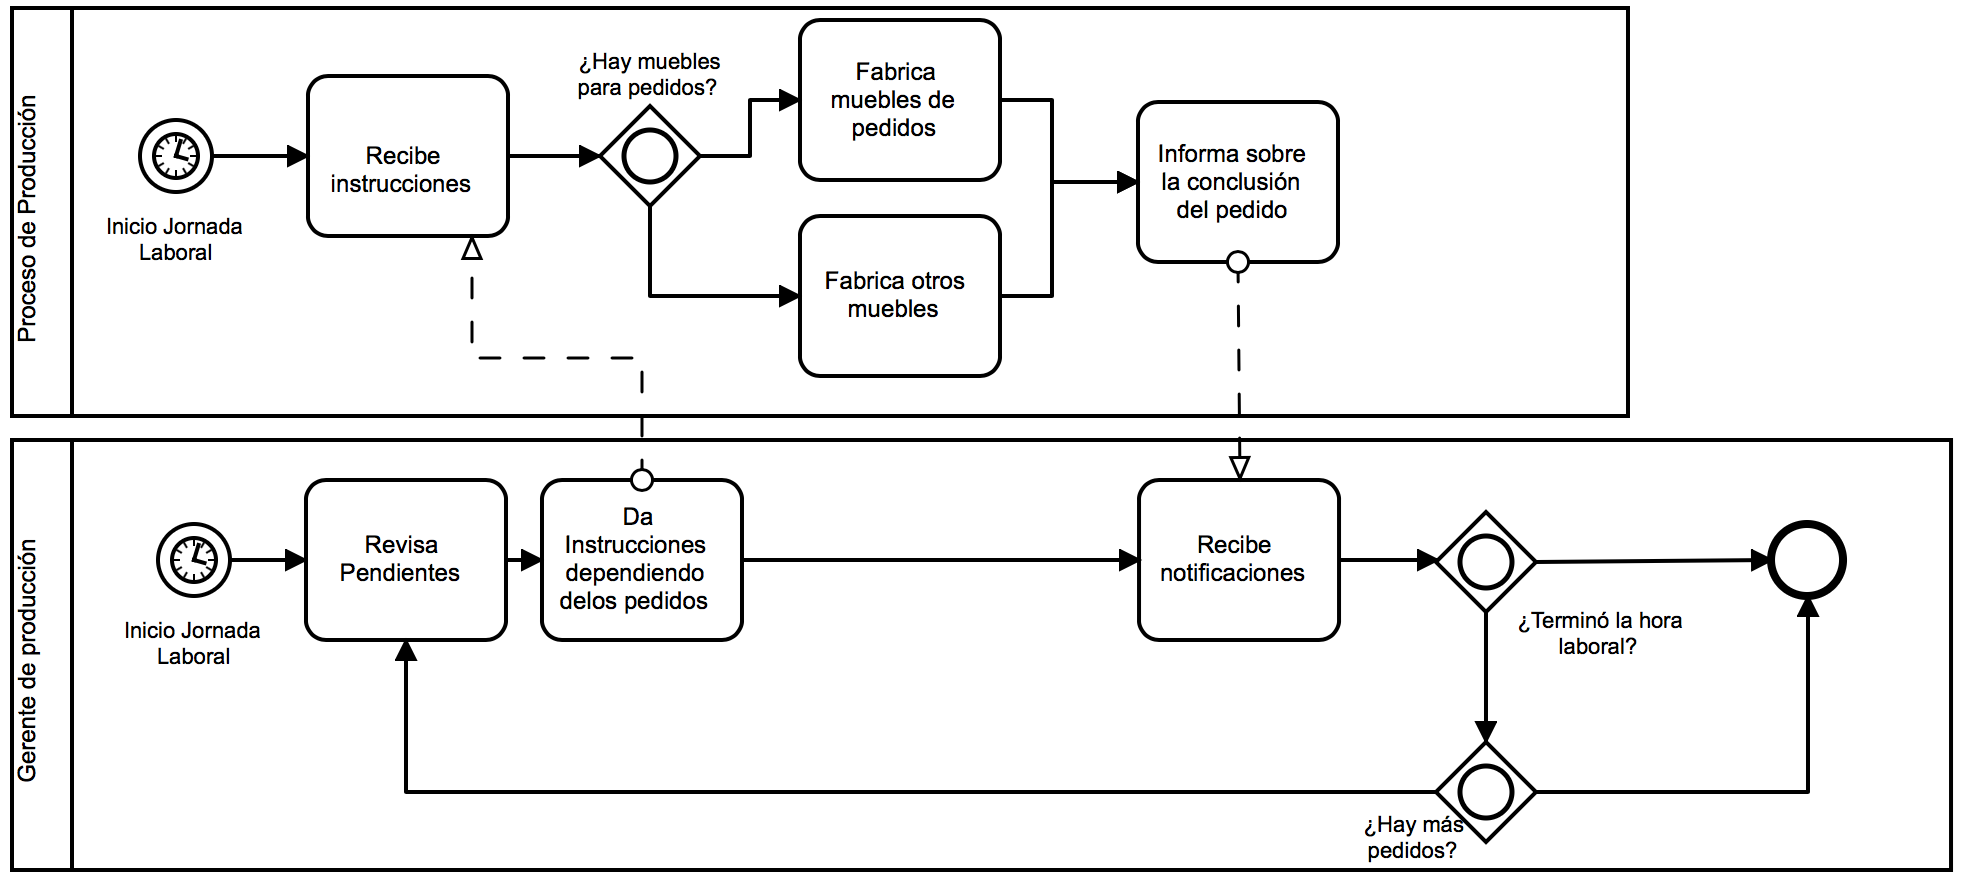
\includegraphics[width=.8\textwidth]{images/proceso3}
		\caption{PROCM-01 Nombre del proceso}
		\label{fig:proceso3}
	\end{center}
\end{figure}

\begin{description}
	\item[Descripción:] ...
	\item[Entradas:] \cdtEmpty
        \begin{itemize}
			\item ...
        \end{itemize}
	\item[Salidas:] \cdtEmpty
        \begin{itemize}
			\item ...
        \end{itemize}	
    \item[Mejoras esperadas:] Liste las mejoras que espera obtener tras la implementación del sistema.
    \item[Reglas de negocio:] \hyperlink{BR05}{BR05}, \hyperlink{BR8}{BR8}.
    \item[Casos de uso:] \hyperlink{CU3.4}{CU 3.4 Login}, \hyperlink{CU 4.3}{ CU 4.3 Consultar productos}.
\end{description}

%\input{proc/proc-m02.tex}
%\input{proc/proc-m03.tex}
%\input{proc/proc-m04.tex}

